\documentclass[11pt]{article}
\usepackage{graphicx} % Required for inserting images
\usepackage{subcaption}
\usepackage[letterpaper, margin=1in]{geometry}
\usepackage{url}
\usepackage[round,authoryear]{natbib}
\usepackage{hyperref}
\usepackage{doi}
\usepackage{enumitem}
\usepackage{booktabs,tabularx,multirow}
\usepackage{amsmath}

\newcommand{\figref}[1]{Fig.~\ref{#1}}

\title{Development of a Data-Assimilative Digital Twin for Wave Energy Converters Using Field, Laboratory and Numerical Data}

\date{}

\begin{document}
\maketitle{}

\section*{Abstract}
This project will develop a data-assimilative digital twin framework for wave energy converter (WEC) design, leveraging existing data sets available to the Pacific Marine Energy Center (PMEC) community. This will include the integration of PacWave environmental wave measurements, Hinsdale tank-test datasets for WECs; physics-based models and WESRF Power Take-Off (PTO) testing data.~Existing data, workflows and requested computing resources will support calibration, independent validation, state estimation and uncertainty assessment.~A reusable workflow will connect field wave inputs, hydrodynamic simulations and physical tank and PTO testing.~Outputs will include device-motion estimates, PTO responses, power predictions and model diagnostics.~The framework will support performance assessment under representative ocean conditions and provide a foundation for future operational prediction and control optimization research.
\section{Project Overview and Research Opportunity}
Digital twins are virtual representations of physical systems that can be used to simulate and optimize the system's behavior.~Within a Wave Energy Converter (WEC) system, a digital twin can help in understanding the complex interactions between the ocean environment, the WEC itself, and its control systems.~In a digital twin framework experimental data is used to calibrate and validate numerical models, which can then be used to predict the behavior of the physical system under different conditions.~This understanding is crucial for improving the design, operation and maintenance.
\par
This project proposes to develop a data-assimilative digital twin for WECs that connect ocean wave measurements, laboratory experiments and numerical simulations to predict device response and power conversion across scales.~PMEC is uniquely positioned through its collaborations and direct access to data from PacWave, one of the few pre-permitted ocean WEC testing sites in the world, alongside the O.H. Hinsdale Wave Research Laboratory and the linear test bed at WESRF.~The framework shown in~\figref{flowchart} will combine full-scale wave data from PacWave, scaled WEC hydrodynamic tank-tests at Oregon State University’s Wave lab and power take-off (PTO) bench experiments at WESRF to create a comprehensive model of WEC behavior.~Measured wave conditions from PacWave will be scaled to laboratory conditions and used as inputs to physics-based WEC models to predict device motions and hydrodynamic forces.~Measurements from Hinsdale wave-tank experiments and WESRF PTO tests will then be combined with the numerical predictions through data assimilation to improve estimates of device response, calibrate selected model parameters and assess prediction uncertainty.~Building on existing numerical tools and WESRF’s force/position driven and coupled testing capabilities for full-scale WECs, the project will establish and validate a generalized, reusable workflow linking tank testing, hydrodynamic simulation with physical PTO testing.~Possibility of integrating ``NVIDIA Omniverse'' to provide a shared 3D environment for the digital twin will be explored.~The resulting framework will support assessment of loads on devices, dynamics and power output under representative ocean conditions.~This workflow will provide a foundation for future integration of operational measurements from deployed devices.
\begin{figure}[t!]
    \centering
    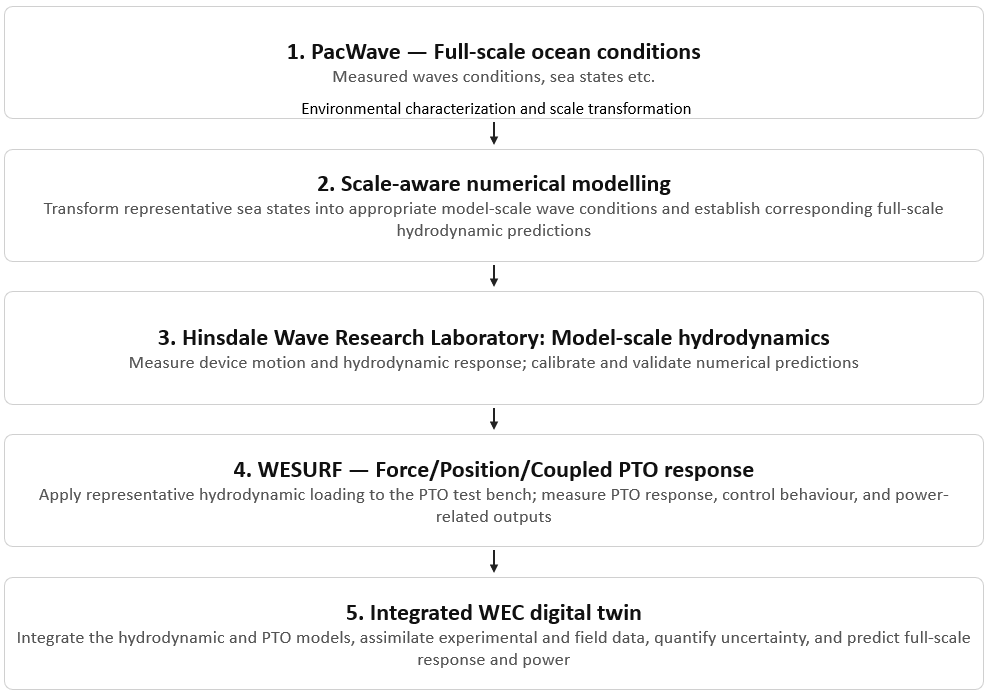
\includegraphics[width=1\textwidth]{flowChart.png}
    \caption{Framework for the proposed data-assimilative digital twin for wave energy converters.}
    \label{flowchart}
\end{figure}
\section{Previous Research and Integration Gap}
Development of digital twins for WECs has gained significant attention in recent years due to the increasing need for accurate and reliable prediction of device performance under real-world conditions.~The wave resource data at~\cite{pacwave2026} was characterized by~\cite{Dunkle2020PacWave}.~\cite{Robertson2022WECSize} examined how spectral conditions at PacWave and other sites influence device-size-dependent energy production and variability.~At field scale,~\cite{O} combined deployment measurements with PTO dynamometer data to improve modelling of a tethered-heave-plate WEC, incorporating generator inertia and measured power-conversion behaviour.~\cite{Ali2025SurgePitch, ali_subharmonic_2026}~in several tank-testing campaigns at OSU investigated the behavior of submerged-WEC's under various conditions.~Nonlinear surge–pitch coupling and subharmonic excitation was investigated respectively in these studies, highlighting the importance of considering nonlinear effects in WEC modeling.~\cite{McConnell2025HybridMooring,McConnell2026HybridFramework} developed and experimentally evaluated real-time hybrid approaches for WEC mooring dynamics using Hinsdale Wave Research Laboratory and PTO bench experiments at WESRF. Additionally, the OSU–Sandia–Evergreen FOSTWIN platform offers both a physics-based WEC-Sim model and a model identified from Hinsdale experimental data for controller development~\cite{FOSTWINDigitalTwin}.~Collectively, these studies provide the data and methodologies to motivate the proposed integration of PacWave field wave conditions, tank-validated hydrodynamics and physical PTO testing within a reusable data-assimilation workflow.

Outside the Pacific Marine Energy Center (PMEC), similar efforts are being made to develop digital twins for wave energy converters.~\cite{Dizon2024FieldValidation} evaluated WEC-Sim and Gazebo models of the deployed MBARI two-body WEC against field measurements across 56 observations, comparing piston velocity, motor speed, and electrical power; the Gazebo model was intended to serve as a digital twin. Previous research provides complementary foundations for WEC digital twins through experimental model identification, field validation, and coupled PTO testing.~\cite{giorgi_identification_2019} used six experimental  datasets to identify and validate efficient linear and nonlinear hydrodynamic models, demonstrating how laboratory measurements can inform predictive models.~\cite{lawal_ai-driven_2026} discuss AI-driven digital twins for wave energy systems, while~\cite{katsidoniotaki_digital_2022} developed a CFD-derived surrogate for rapid prediction of extreme mooring loads. Related computational approaches include nonlinear response prediction using multiple-input operator networks by~\cite{zhang_multiple-input_2025}, CFD-coupled reinforcement learning for adaptive PTO control by~\cite{liang_environmental-sensing_2024}, and data-driven control methods reviewed by~\cite{pasta_towards_2023}. 
For physical PTO testing,~\cite{Bracco2015ISWECHIL} coupled an ISWEC gyroscope and generator test rig with a numerical hydrodynamic model through hardware-in-the-loop simulation, while~\cite{Bacelli2019TankBench} demonstrated control testing through complementary dry-bench and wave-tank experiments. Together, these studies motivate a framework connecting measured ocean-wave conditions, tank-validated hydrodynamics, and physical PTO response. 

The proposed project will build on these approaches by developing a reusable workflow that explicitly assimilates laboratory measurements to update model estimates and assess prediction uncertainty across the hydrodynamic and PTO testing stages.

\section{Research Objectives and Expected Outcomes}
The main objectives of this project are:
\begin{enumerate}[noitemsep]
    \item Identify the representative wave conditions derived from PacWave measurements.
    \item Organize the existing tank-testing and PTO (Pneumatic) datasets into a documented structure that preserves device geometry, scale, instrumentation, wave conditions and PTO settings.
    \item Identify the most appropriate numerical models (WEC-Sim, CFD) that reproduce selected laboratory experiments and validate their predictions against independent datasets. 
    \item Develop and evaluate a data-assimilation method that uses measured device response to update estimated states and selected model parameters. 
    \item Integrate the resulting hydrodynamic model with WESRF’s physical PTO testing capabilities and evaluate the coupled response. 
\end{enumerate}
Expected outcomes include generation of dataset, validated baseline and updated models, a documented coupled simulation and testing workflow and an assessment of prediction accuracy and uncertainty.~Success will be demonstrated through reproducible comparisons of device motion, PTO displacement/velocity, measured loads and power metrics.

\section{Research Approach: Connecting Field, Tank, and PTO Data}
Continuous PacWave wave measurements will define representative environmental conditions for numerical simulations and laboratory tests with relevant scaling. Existing tank datasets from~\cite{ali_subharmonic_2026, Beringer2025IrregularUncertainty, Beringer2026RegularUncertainty} and collaborators will support hydrodynamic model calibration and independent validation.~The PTO system that was used in the tank testing and the dyployed SubWEC during this test are shown in~\figref{fig:pto} and~\figref{fig:osutank}, respectively and the linear test bed that is used for PTO testing is shown in~\figref{fig:linearbed}.~Each dataset will retain its original geometry, scale and test configuration.~Numerical simulations will use the measured laboratory waves as input to the models.~Comparison of the wave parameters, relative body motion and measured PTO quantities will be made to assess model performance.~Ali’s studies will inform assessment of nonlinear coupled motions, while Beringer’s uncertainty methods will help distinguish model discrepancies from experimental variability.
\begin{figure}[t!]
    \centering
    \begin{subfigure}[b]{0.36\textwidth}
        \centering
        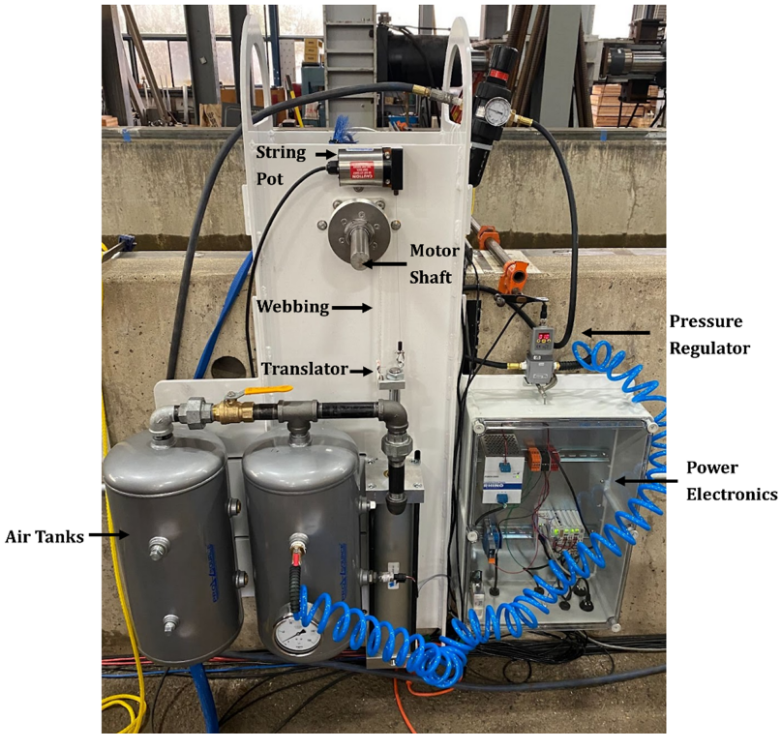
\includegraphics[width=\textwidth]{pto.png}
        \caption{The PTO system used in the tank testing of the SubWEC}
        \label{fig:pto}
    \end{subfigure}
    \hfill
    \begin{subfigure}[b]{0.34\textwidth}
        \centering
        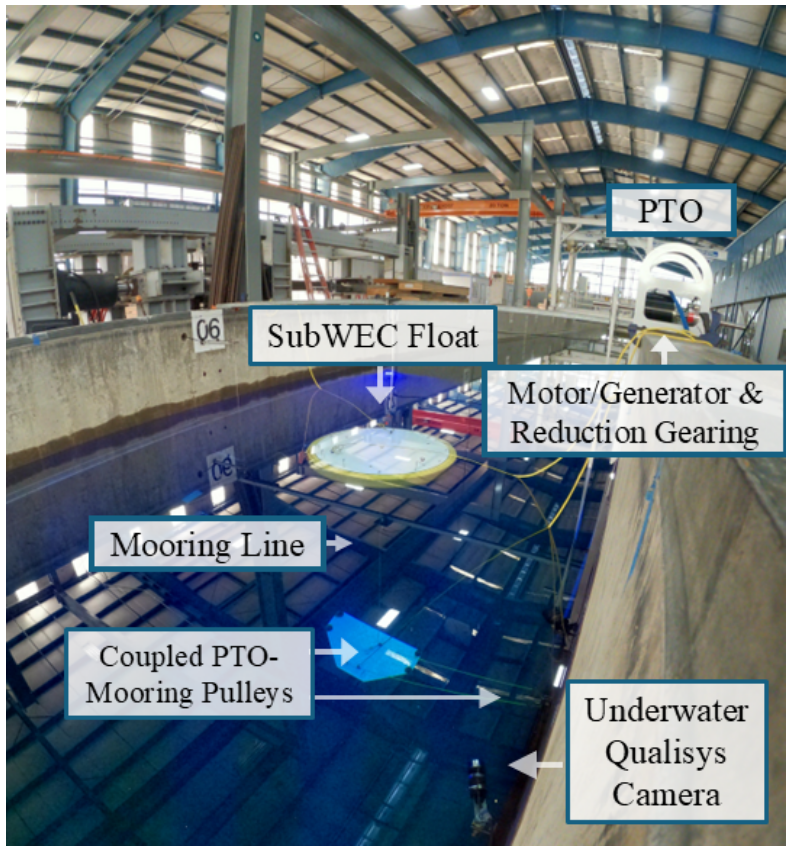
\includegraphics[width=\textwidth]{OSUtank.png}
        \caption{SubWEC in the Large Wave Flume (LWF) at OSU}
        \label{fig:osutank}
    \end{subfigure}
        \hfill
    \begin{subfigure}[b]{0.28\textwidth}
        \centering
        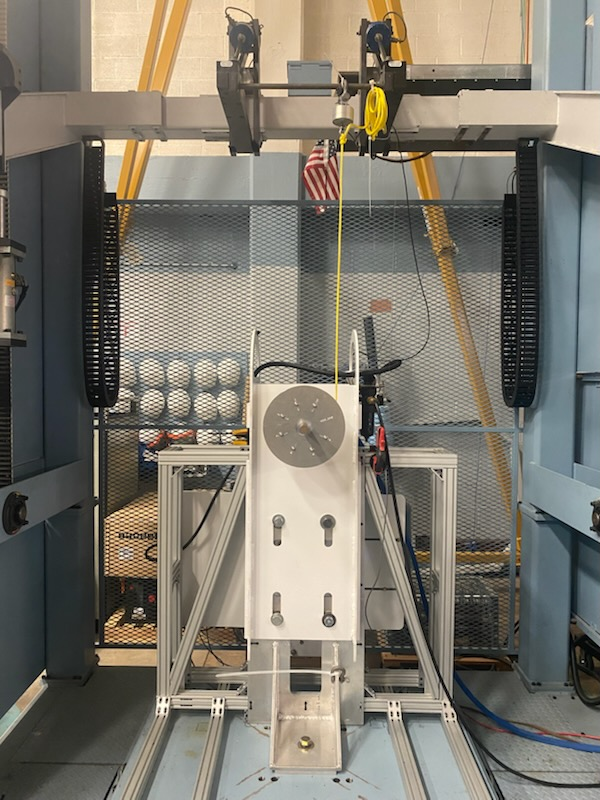
\includegraphics[width=\textwidth]{LTB-WESRF.png}
        \caption{The linear test bed at WESEF Lab at OSU}
        \label{fig:linearbed}
    \end{subfigure}
    \caption{Experimental facilities supporting the proposed digital-twin workflow.}
    \label{fig:experimental-facilities}
\end{figure}
PTO modelling and testing will build on~\cite{Kim2025InstantaneousFrequency} previous WESRF work and the laboratory’s existing force/position and coupled testing capabilities.~Available bench records will characterize PTO behavior and the numerical models will exchange force/motion information information with the physical PTO. McConnell and Bosma’s hybrid simulation experience will inform communication, actuator tracking and delay assessments. The resulting interfaces and procedures will be documented as a reusable workflow.

The data-assimilation framework will initially be tested using existing laboratory datasets, and then integrated with real-time measurements from PTO bench tests.~A state estimator will combine model predictions with motion and PTO measurements to update estimated positions and velocities. Measurement and model uncertainty will inform the updates. Performance will be assessed against uncalibrated and calibrated models without assimilation, using independent cases.

NVIDIA Omniverse will be evaluated as a common visualization environment connecting WEC geometry, experimental measurements, and numerical predictions. An OpenUSD representation of the device and selected test configurations will support synchronized replay of existing tank and PTO bench datasets alongside simulated responses.

\section{Computational Readiness and Resource Requirements}
Computational readiness is dependent on several years of numerical workflows, accessible experimental datasets and established laboratory hardware.~Available modelling tools include frequency and time-domain WEC-Sim, ANSYS-Aqwa and ProteusDS workflows and OpenFOAM CFD capabilities, supported by MATLAB and Python processing tools.~Existing tank datasets from testing of LUPA, SubWEC and FOSWEC and prior WESRF testing reduce dependence on a new experimental campaign to initiate this project.~The first project stage will document dataset availability, calibration records and model validations.~Advanced computing will support parallel hydrodynamic parameter studies, selected CFD investigations of nonlinear response and ensemble calculations used to examine uncertainty.~Efficient linear models will support repeated estimation and coupled testing, while higher-fidelity calculations will be targeted at cases where simpler models show unresolved discrepancies.~Before larger workloads are scheduled the computing requirements like processor time, memory and storage will be estimated through benchmark runs.
\section{Work Plan, Milestones, and Validation}
A phased twelve-month plan, reuse of existing facilities and focused personnel support will keep the scope and resource requirements manageable.~The project will be completed over twelve months.~Proposed activities and milestones are summarized in Table~\ref{tab:project_work_plan}. The first four months will focus on dataset inventory, model configuration, and baseline validation. Months five through eight will develop and evaluate the data-assimilation framework, including parameter identifiability and uncertainty assessment. The final four months will integrate the hydrodynamic model with WESRF PTO testing, validate the coupled workflow, and assess full-scale predictions.

\begin{table}[t!]
\centering
\caption{Monthly project activities, milestones, and three research phases.}
\label{tab:project_work_plan}
\small
\renewcommand{\arraystretch}{1.25}

% Adjust 4.2cm if needed to match the height of each four-month block.
\newcommand{\phasebrace}[1]{%
  $\left.\rule[-2.1cm]{0pt}{4.2cm}\right\}
  \begin{gathered}
    \text{Phase}\\[-2pt]
    \text{#1}
  \end{gathered}$%
}

\begin{tabularx}{\textwidth}{
    @{} c c
    >{\raggedright\arraybackslash}X
    >{\raggedright\arraybackslash}X @{}
}
\toprule
\textbf{Month} & \textbf{Phase} & \textbf{Main activities}
& \textbf{Milestone / deliverable} \\
\midrule

1 & \multirow{4}{*}{\phasebrace{I}}
& Inventory and quality-check PacWave, Hinsdale, and WESURF
datasets; select test cases.
& Dataset inventory and calibration--validation split. \\

2 &
& Configure hydrodynamic models using measured tank-wave inputs.
& Reproducible baseline simulations. \\

3 &
& Compare predicted and measured motions, spectra, and
available PTO quantities.
& Baseline accuracy and discrepancy assessment. \\

4 &
& Calibrate selected parameters and evaluate withheld tank cases.
& Baseline model validation report. \\

\midrule

5 & \multirow{4}{*}{\phasebrace{II}}
& Develop a state estimator using recorded laboratory measurements.
& Initial data-assimilation implementation. \\

6 &
& Evaluate estimation and prediction accuracy; assess
parameter identifiability.
& Comparison with models without assimilation. \\

7 &
& Perform targeted CFD and ensemble studies to assess uncertainty.
& Model and prediction uncertainty assessment. \\

8 &
& Evaluate assimilation on independent cases and characterize
PTO behaviour using bench records.
& Evaluated assimilation framework and coupling requirements. \\

\midrule

9 & \multirow{4}{*}{\phasebrace{III}}
& Integrate the hydrodynamic model with WESURF interfaces;
conduct recorded-input tests.
& Verified communication, timing, and actuator tracking. \\

10 &
& Conduct coupled simulation--PTO tests and independent validation.
& Validated coupled workflow and repeatability assessment. \\

11 &
& Simulate representative PacWave sea states; assess uncertainty
and scaling limitations.
& Laboratory-informed full-scale predictions. \\

12 &
& Finalize software, documentation, datasets, and manuscripts.
& Reusable workflow, final report, and manuscripts. \\

\bottomrule
\end{tabularx}
\end{table}

\section{Impact Readiness and Pathway to External Funding}
The project will increase the scientific value of existing investments in PacWave, Hinsdale tank experiments and WESURF PTO testing by connecting their outputs within a reproducible modelling framework. Its immediate contribution will improve understanding of how hydrodynamic response, PTO behaviour and measurement uncertainty influence WEC performance predictions. A reusable workflow could reduce repeated model-setup effort and help researchers identify which additional experiments or higher-fidelity computations are most needed.~The project will also provide practical training to the intern and research personal in marine hydrodynamics, scientific computing, experimental data processing, state estimation and hardware–software integration.~The training will be complemented by hands-on experience with the tools and techniques needed for successful implementation of the digital twin approach.~Documented examples and datasets suitable for release will support student research and future capstone activities.
\par
The validated workflow and initial results will provide evidence for subsequent proposals to DOE water-power programs, NSF, ONR and other relevant sponsors. Future research could extend the framework to deployed-device measurements, additional PTO technologies, controller evaluation, and load monitoring.~This award will establish the computational and experimental foundation needed to pursue those applications credibly.~Advanced computing will enable extensive parameter studies, uncertainty quantification and targeted high-fidelity simulations, allowing exploration of conditions beyond the practical scope of physical testing.~Coupling those calculations with existing measurements will produce a stronger basis for future funding proposals, publications, and collaborations focused on reliable wave-powered ocean systems.
\par
Huang Complex computing resources will enable parallel parameter studies, uncertainty ensembles and targeted high-fidelity simulations.~More reliable performance assessment will reduce development costs and support wave-powered ocean monitoring and other applications for communities.~A reusable digital twin workflow will strengthen competitive external funding proposals, train researchers and expand OSU’s marine-energy research capabilities.~A focus on renewable energy and computational research will support the proposal’s alignment with PWS priorities.
% \nocite{*}
\bibliographystyle{plainnat}
\bibliography{references}

\end{document}